\documentclass[english]{scrartcl}
\pagenumbering{arabic}
\usepackage[utf8]{inputenc}
\usepackage[english]{babel}
\usepackage{amsmath}
\usepackage{amsfonts}
\usepackage{amssymb}
\usepackage{fancyvrb}
\usepackage{xspace}
\usepackage{refstyle}
\usepackage{hyperref}
\usepackage{listings}
\usepackage{enumitem}
\usepackage{graphicx}
\usepackage{placeins}
\usepackage{subcaption}
\usepackage{caption}
\usepackage{courier}
\usepackage{microtype}
\usepackage[htt]{hyphenat}

% ============================================================
% Style for monospace text
\lstset{basicstyle=\ttfamily,breaklines=true}

% ============================================================
% Markup macros for proof-reading
\usepackage{ifthen}
\usepackage[normalem]{ulem} % for \sout
\usepackage{xcolor}
\newcommand{\ra}{$\rightarrow$}
\newboolean{showedits}
\setboolean{showedits}{true} % toggle to show or hide edits
%\setboolean{showedits}{false} % toggle to show or hide edits
\ifthenelse{\boolean{showedits}}
{
	\newcommand{\ugh}[1]{\textcolor{red}{\uwave{#1}}} % please rephrase
	\newcommand{\ins}[1]{\textcolor{blue}{\uline{#1}}} % please insert
	\newcommand{\del}[1]{\textcolor{red}{\sout{#1}}} % please delete
	\newcommand{\chg}[2]{\textcolor{red}{\sout{#1}}{\ra}\textcolor{blue}{\uline{#2}}} % please change
}{
	\newcommand{\ugh}[1]{#1} % please rephrase
	\newcommand{\ins}[1]{#1} % please insert
	\newcommand{\del}[1]{} % please delete
	\newcommand{\chg}[2]{#2}
}
% ============================================================
% Put edit comments in a really ugly standout display
%\usepackage{ifthen}
\usepackage{amssymb}
\newboolean{showcomments}
\setboolean{showcomments}{true}
%\setboolean{showcomments}{false}
\newcommand{\id}[1]{$-$Id: scgPaper.tex 32478 2010-04-29 09:11:32Z oscar $-$}
\newcommand{\yellowbox}[1]{\fcolorbox{gray}{yellow}{\bfseries\sffamily\scriptsize#1}}
\newcommand{\triangles}[1]{{\sf\small$\blacktriangleright$\textit{#1}$\blacktriangleleft$}}
\ifthenelse{\boolean{showcomments}}
%{\newcommand{\nb}[2]{{\yellowbox{#1}\triangles{#2}}}
{\newcommand{\nbc}[3]{
 {\colorbox{#3}{\bfseries\sffamily\scriptsize\textcolor{white}{#1}}}
 {\textcolor{#3}{\sf\small$\blacktriangleright$\textit{#2}$\blacktriangleleft$}}}
 \newcommand{\version}{\emph{\scriptsize\id}}}
{\newcommand{\nbc}[3]{}
 \renewcommand{\ugh}[1]{#1} % please rephrase
 \renewcommand{\ins}[1]{#1} % please insert
 \renewcommand{\del}[1]{} % please delete
 \renewcommand{\chg}[2]{#2} % please change
 \newcommand{\version}{}}
\newcommand{\nb}[2]{\nbc{#1}{#2}{orange}}
\newcommand{\here}{\yellowbox{$\Rightarrow$ CONTINUE HERE $\Leftarrow$}}

\newcommand\rev[2]{\nb{TODO (rev #1)}{#2}} % reviewer comments
\newcommand\fix[1]{\nb{FIX}{#1}}
\newcommand\todo[1]{\nb{TO DO}{#1}}
\newcommand\meta[1]{\nbc{META}{#1}{purple}}
\newcommand\jr[1]{\nbc{JR}{#1}{orange}}
\newcommand\nes[1]{\nbc{nes}{#1}{blue}}
\newcommand\on[1]{\nbc{ON}{#1}{red}} % add more author macros here
\newcommand\ewe[1]{\nbc{EWE}{#1}{olive}} % add more author

% ============================================================

\newcommand{\bs}{\symbol{'134}} % backslash
\newcommand{\us}{\symbol{'137}} % underscore
\newcommand{\ie}{\emph{i.e.}\xspace}
\newcommand{\eg}{\emph{e.g.}\xspace}
\newcommand{\etal}{\emph{et al.}\xspace}

\newcommand{\DD}{Dood\-le\-De\-bug\xspace}
\newcommand{\Doodle}{\texttt{Doo.\-dle}\xspace}
\newcommand{\println}{\texttt{Sys\-tem.\-out.\-println}\xspace}

% ============================================================

\begin{document}
\title{DoodleDebug}
\author{Cedric Reichenbach}
\subtitle{A shot-gun marriage between System.out.println and object inspectors}
\maketitle

\begin{abstract}
Developers need effective ways to inspect and explore the run-time state of programs they are developing and debugging.  Modern debuggers and object inspectors are powerful tools, but they can only be used to explore specific points in the execution where breakpoints have been set. As a result, developers often resort to inserting ``print statements'' in code to log the state at multiple points in the execution. Print statements, however are a ``poor man's debugger'', since their output is static and cannot be further explored.
We propose to combine the simplicity of print statements with the graphical sophistication and interaction of modern debugging tools.
\DD is a simple API modeled loosely after Java's \println. Objects that are ``printed'' generate graphical views that can be further explored, and can also be used to navigate back to source code in the IDE.
We introduce \DD and present the results of a usability study that shows that \DD can be very effective for common debugging tasks.
\end{abstract}

\section{Introduction}

To understand and debug a program, developers rely on tools to track its runtime states during execution.
One method is to insert print statements like \println in Java.
This method is quick and allows programmers to compare different states in time of a specific object.
However, this output is static and comes with a couple of conceptual restrictions. On the one hand, the level of detail is hardcoded through the textual representations of objects.
If a developer decides for a simple and clear way of representation, they will need to rewrite their code for any further inspection and re-run the program after every change, which is particularly a problem in a long-running program.
If they initially choose a detailed and verbose object representation, the output will grow and become tedious to read.

Another drawback of textual representation is caused by the simplicity of plain text.
Its one-dimensional nature prevents the user from encapsulating multidimensional object representations.
In other words, objects using line breaks in their \texttt{toString} representation cannot be nested consistently, since switching to a new line is always a final operation.

The other half of the two most widely used debugging tools is the family of debuggers~\cite{Kras88a}.
When utilizing a debugger, a program can be stopped at a specific point of its execution, allowing developers to inspect any detail of this very state.
A clear advantage over textual output is the ability to inspect objects on demand.
Information is only displayed as soon as the user asks for it, nevertheless available without re-running the program.
As McConnell states in Code Complete\cite[p. 539]{McCo04a}, debuggers help to avoid bad practices caused by debugging with \println, like scattering print statements randomly throughout a program.
The drawbacks of debuggers arise from the fact that their inspector is always bound to a specific point in time and therefore makes it impossible to directly compare different states of the same object.

\DD combines the power of the above mentioned tools, erasing the conceptual problems coming with them.
Its output is generated through an API taking its cue from \println.
A developer simply needs to call \Doodle(object) to doodle any object type.
Hence, \DD's usage, as well as that of \println, is orthogonal to the control flow of debuggers; they can be used in combination.
A debugger can step over one \Doodle statement at a time and new doodles instantly appear.
On the other hand, when a program is held still by a debugger, the user can make it evaluate any custom expression, including \Doodle statements.

For simple customization of object representations, a class can implement the \texttt{Doodleable} interface which contains 2 methods, \texttt{doodleOn} and \texttt{summarizeOn}.
In contrast to Java's \texttt{toString}, there are two methods, allowing developers to define representations on two levels of detail.
This distinction allows inspection of objects directly in the output window.

As output format, \DD uses the web standards HTML and CSS to enhance formatting possibilities over simple text.

The functionality \DD offers consists of the following main points:
\begin{enumerate}
\item A log of all states of an object when it was doodled in the past
\item Zooming into one particular state in the log for more detail
\item A lean API for doodling objects
\end{enumerate}

\begin{figure}[h]
	\centering
	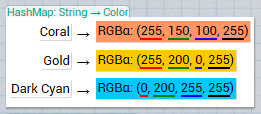
\includegraphics[width=0.5\linewidth]{img/Plugin_Map-Color.png}
	\caption{Doodle of a map from strings to colors with built-in renderings only.}
	\figlabel{plugin_map-color}
\end{figure}

\section{Features}
This section outlines the major features and properties of DoodleDebug from a user's perspective.
Different parts are ordered by importance we gave them during development.

\subsection{Lean API}
The \DD API is lean.
It features three ways for developers to interact with it, though most will only ever use the first two.
\begin{itemize}
\item The \texttt{Doo.dle(Object)} method as a drop-in replacement for \println
\item The \texttt{Doodleable} interface and the associated interface \texttt{DoodleCanvas}, in which objects can define simple custom representations
\item The \texttt{RenderingPlugin} interface, which allows developers to provide powerful custom renderings for any type, based on HTML and CSS; source code access is not required here.
\end{itemize}
Altogether, \DD features no more than 10 public methods.

\subsection{Configuration-Free}
A key question in the design of a user interface is the level of configurability exposed to users.
Highly customizable solutions may be better for power users who are very familiar with the software in question.
Other users may always remain on default settings, independent of their suitability.
We followed the advice of Norman\cite[p. 199-200]{Norm88a} and Buxton\cite[p. 102]{Buxt07a}, which says not to treat everyone as a designer, but rather take away design decisions from users by creating sophisticated defaults.
As a consequence, there is no settings dialogue or file for \DD.

\subsubsection{Smart Scrolling}
In general, an output console can either move its view port to the bottom when new content is appended or stay where it was before.
\DD implements the scrolling behavior of MUSHClient\footnote{\url{http://www.gammon.com.au/mushclient/}} and mIRC\footnote{\url{http://www.mirc.com}}:
The viewport will only be moved to the bottom if it already was there before new content was added.
If the user doesn't scroll away from the bottom, they will benefit from notifications about new doodles.
On the other hand, users can scroll up to an old doodle without being bounced away when new objects are doodled.

\subsubsection{Notifications}
\seclabel{smart-focus}
When new objects are doodled, \DD autonomously decides whether to set focus to the \DD output view for user notification or not.
The crucial factor for this decision is the elapsed time since the last doodling.
Focus is gained if more than 4 seconds have passed and always for the first doodle of a program run.

When debugging a program with many output events per second, like a game, there is no sense in always notifying the user.
Either they keep their attention on the output as they see it's rapidly changing, or they work somewhere else in the UI and don't want to be pulled back every time.
During our study (\secref{study}), subject Echo manually disabled such notifications of the Eclipse console, complaining about it stealing the focus of the UI part they were working in.

For a program expected to be silent in general, there's no need for suppressing eventual output notifications.
One use case could be an unplanned exception that's caught, but doodled in order to inform the programmer about a possible problem.


\subsection{Inspection of Doodled Objects}
To avoid the trade-off between detail level and compactness, we implemented the principle of \emph{semantic zoom} along with \DD:
Every object features two levels of detail for its rendering.
Objects that are nested into others are not graphically scaled down, nor removed, but rendered in their summarized, less detailed  version.

Object doodles are divided into levels, based on their nesting depth.
An object provided in the \Doodle call has level 0.
Every object directly referenced inside this one renders at level 1, those referenced from level 1 render at level 2 and so on.

In \DD, objects rendered at nesting levels 0 and 1 are rendered with full detail; objects at nesting level 2 show their summarized version.
Clicking on a level 1 object opens a popup window only showing this very object, but with more detail since it's at the new nesting level 0 now.
Level 1 objects in this window can again be clicked in order to inspect those.
This can be repeated until any end node of the doodling graph is reached, \ie one that has no references.
\Figref{addressbook_whole} shows a doodled address book (at level 0) containing several contacts (at level 1). Clicking on one of them creates a pop-up window, moving the respective contact object to new level 0 (\Figref{addressbook_contact}).

Navigation between nesting layers inside a pop-up is aided with bread crumbs~\cite[p. 76-78]{Krug00a}, which traces the currently inspected branch of the object graph (\figref{breadcrumbs}).
Any parent doodle in this trace can be clicked to jump to it directly.
When zooming out of the graph this way, the just visited branch is still visible in the breadcrumbs area until the user turns into a new path.

\begin{figure}[h]
	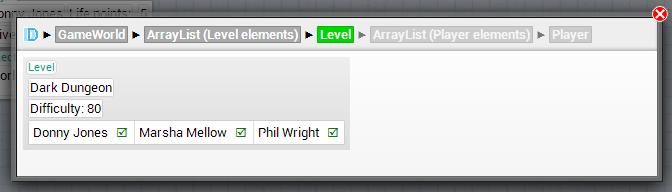
\includegraphics[width=\linewidth]{img/breadcrumbs.png}
	\caption{The labels at the top are \emph{bread crumbs}. The developer is currently looking at a \texttt{Level} object, which is the member of an ArrayList, which is the member of a \texttt{GameWorld}. The object that was doodled was the \texttt{GameWorld} object. The developer was previously zoomed in to player but zoomed out again to Level.}
	\figlabel{breadcrumbs}
\end{figure}

\subsubsection{Tracking an Object Over Time}

Thanks to \DD's inspection feature, the summarized representation of an object can be kept rather terse.
As an example, the state of a game can be doodled on every update cycle like in \figref{game_long-list}.
A developer observing this output may be interested in more detail of one particular state, which can be done by clicking on parts of it, resulting in a pop-up (\figref{game_last-state}).

The program code defining a \texttt{Player}'s rendering looks as follows:
\begin{lstlisting}
public class Player implements Doodleable {
	public void doodleOn(DoodleCanvas c) {
		c.draw(name);
		c.newLine();
		c.draw("Alive?");
		c.draw(isAlive);
		c.newColumn();
		c.draw("Life points:");
		c.draw(lifePoints);
	}

	public void summarizeOn(DoodleCanvas c) {
		c.draw(name);
		c.draw(isAlive);
	}
}
\end{lstlisting}

\begin{figure}[h]
	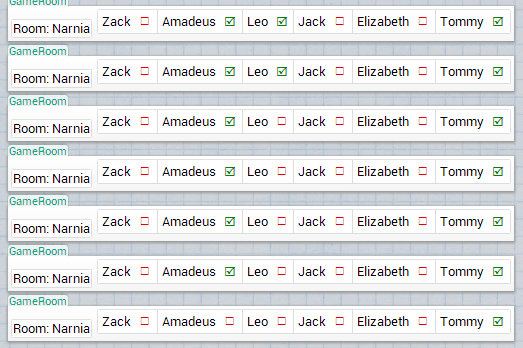
\includegraphics[width=\linewidth]{img/game_long-list.png}
	\caption[Example of a chronological sequence: Game]{A DoodleDebug console showing the doodles of \texttt{GameRoom}s. The boxes beside each are summarized booleans and indicate if the player is alive.}
	\figlabel{game_long-list}
\end{figure}

\begin{figure}[h]
	\centering
	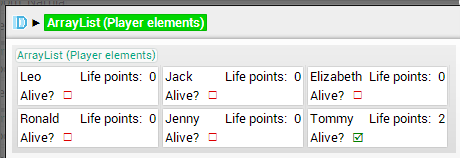
\includegraphics{img/game_last-state.png}
	\caption[Example of a chronological sequence: Detailed player list]{Details of a \texttt{GameRoom} from \Figref{game_long-list}.}
	\figlabel{game_last-state}
\end{figure}

\begin{figure}[h]
\begin{subfigure}{0.42\linewidth}
	\centering
	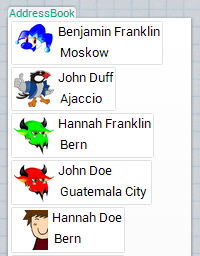
\includegraphics{img/AddressBook_whole.png}
	\caption[AddressBook visualization]{An address book only showing the summaries of its addresses. Clicking reveals the details in \figref{addressbook_contact}.}
	\figlabel{addressbook_whole}
\end{subfigure}
\hspace{0.03\linewidth}
\begin{subfigure}{0.55\linewidth}
	\centering
	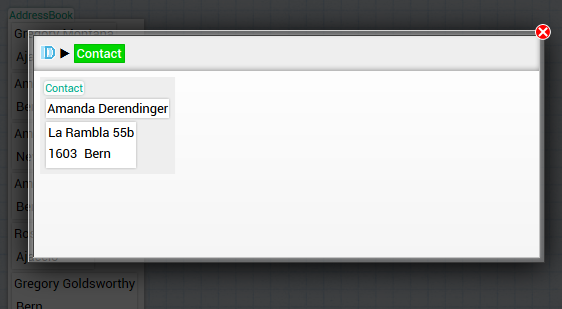
\includegraphics{img/AddressBook_contact.png}
	\caption[Contact visualization]{A popup showing the details of an address.}
	\figlabel{addressbook_contact}
\end{subfigure}
\caption{Exposure of a contact object at two different levels of detail.}
\end{figure}

\subsection{Built-in Renderings}
\DD comes with predefined renderings for a number of commonly used data types in Java.
Those include:
\begin{itemize}[noitemsep]
\item Primitives
\item Arrays (same layout as Collections)
\item Booleans (\figref{plugin_boolean})
\item Classes (\figref{plugin_class})
\item Collections (\figref{game_long-list} and \figref{plugin_collections-small})
\item Colors (\figref{plugin_map-color})
\item Images (various types)
\item Maps (\figref{plugin_map-color})
\item Nulls (\figref{plugin_boolean})
\item Objects (default, \figref{fielddoodler-player})
\item Strings
\item Tables (rectangular two-dimensional arrays and collections, \figref{nested-matrix-doodle-debug})
\item Trowables (\figref{plugin_throwable})
\end{itemize}

\begin{figure}[h]
\begin{minipage}[t]{0.4\linewidth}
	\centering
	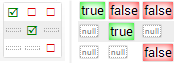
\includegraphics{img/Plugin_Boolean.png}
	\caption{Summarized and detailed renderings of booleans.}
	\figlabel{plugin_boolean}
\end{minipage}
\hspace{0.03\linewidth}
\begin{minipage}[t]{0.57\linewidth}
	\centering
	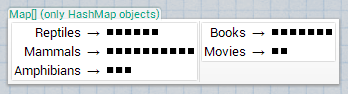
\includegraphics[width=\linewidth]{img/Plugin_Collections-small.png}
	\caption{A doodled array of maps from strings to collections. The collections are rendered as summarized.}
	\figlabel{plugin_collections-small}
\end{minipage}
\end{figure}

\begin{figure}[h]
	\centering
	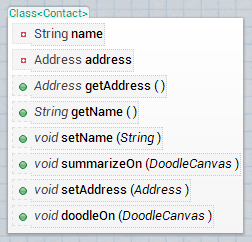
\includegraphics[width=0.5\linewidth]{img/Plugin_Class.png}
	\caption{Rendering of a class object.}
	\figlabel{plugin_class}
\end{figure}

\begin{figure}[h]
\begin{minipage}{.5\linewidth}
	\centering
	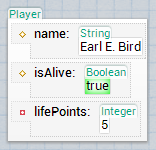
\includegraphics{img/FieldDoodler_player.png}
	\caption{The standard rendering of an object, visualizing all of its fields.}
	\figlabel{fielddoodler-player}
\end{minipage}
\begin{minipage}{.5\linewidth}
	\centering
	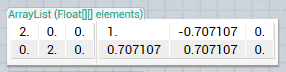
\includegraphics{img/matrix-array.png}
	\caption{\DD's rendering of the same array as shown in \Figref{nested-matrix-problem}}
	\figlabel{nested-matrix-doodle-debug}
\end{minipage}
\end{figure}

\begin{figure}[h]
	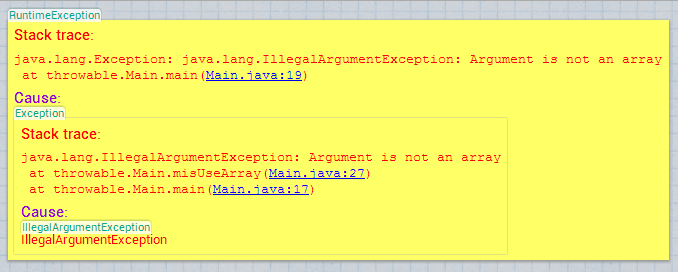
\includegraphics[width=\linewidth]{img/Plugin_Throwable-outermost.png}
	\caption{Rendering of an exception.}
	\figlabel{plugin_throwable}
\end{figure}

\subsection{Customization API}
\DD's API features two API layers for customization, Doodleables and Plugins.
\texttt{Doodleable} customizations are always preferred over plugins when both are available for a type.

\subsubsection{The Doodleable Interface}

As a high-level customization layer, \texttt{Doodleable} utilizes an approach similar to Java's \texttt{toString()} method and targets most use cases since it's a simple and quick solution.
The \texttt{Doodleable} interface features two methods: \texttt{doodleOn(DoodleCanvas)} for a regular representation and \texttt{summarizeOn(DoodleCanvas)} for a simplified and compact version.
Distinguishing between them enables semantic zoom\cite{Wood98a} when inspecting doodles:
instead of geometrically scaling items, they gain more detail when zooming in.

\paragraph{DoodleCanvas}
Instead of creating a string like in \println, both methods receive a \texttt{DoodleCanvas} object for drawing contents on.

\begin{center}
	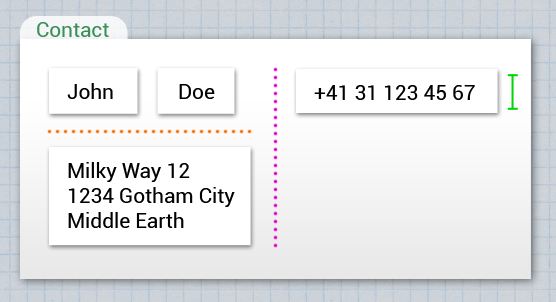
\includegraphics[width=\linewidth]{img/doodleable-example.png}
	\captionof{figure}{Example of a \texttt{Contact} class' \texttt{doodleOn()} method.
Dotted lines visualize the effect of the structuring methods \texttt{newLine()} (orange) and \texttt{newColumn()} (purple).
The green i-beam indicates the final position of the canvas' imaginary cursor.}
	\figlabel{canvas-illustration}
\end{center}

\Figref{canvas-illustration} illustrates how output is generated from a code sample.
The paradigm behind \texttt{DoodleCanvas} adopts the formatting of text in terms of lines and columns.
A virtual cursor starts at the upper-left corner of the canvas.
Drawn objects align one beside each other until a new line is created, which causes the cursor to jump back to the left which one line height offset.
The second formatting option is to create new columns, moving the cursor to a position on top, to the right of the right-most previous object.
\texttt{DoodleCanvas} therefore has three public methods: \texttt{draw(Object)}, \texttt{newLine()} and \texttt{newColumn()}.

\subsubsection{Plugins}
There are cases where implementing the \texttt{Doodleable} canvas is not a satisfying option for developers.
If they don't have access to the source code, there is no (clean) way to add an interface.
Also, the \texttt{Doodleable} API only provides primitive formatting options.

The second layer hooks in on a lower level by allowing users to provide \texttt{RenderingPlugin}s, which are also used internally for \DD's built-in renderings.
At the plugin level, the user can directly control the generation of HTML, CSS, and JavaScript.

\paragraph{Implementing Plugins}
For advanced arrangement or additional features like coloring, \DD includes the option to provide plugins.
They must implement \texttt{RenderingPlugin}, which is most easily done by extending the built-in \texttt{AbstractPlugin}.
Each plugin holds information about the object types it is able to render.
Instead of drawing to a virtual canvas, a plugin receives a html \texttt{Tag} object and renders its own HTML code into this tag.
The principle of semantic zoom is retained through two different methods for different detail levels.
In addition to HTML code generation, plugins have the option to cleanly provide CSS rules and individually adjust class attributes assigned to object doodles.


\section{Design}
For the design of \DD's output, we consulted literature to carefully plan the different project cycles.
As suggested by Buxton\cite[p. 73-76]{Buxt07a}, we decided to start with an initial design phase, which later fades into implementation as soon as a reasonable concept is available.
In particular, we started off by sketching parts of the future user interface with pen and paper and confronted possible users with them.
They were not told what a specific picture would represent, but directly had to state their intuition of what they believed it to be (\figref{sketch-discussion}).
Based on their feedback, we had an estimation of every sketch's quality in terms of intelligibility and could either keep, improve or dismiss it.
This cycle was repeated until our sketches reached a form where they were easily understood by people and we could start implementing.

Since the pen and paper sketches were rough and drafted quickly, the implementation phase initially revealed minor usability problems that had not been obvious in the design phase.
Those were eliminated dynamically, still following Buxtons idea of gradually reducing design while implementation slowly starts.

\begin{figure}[h]
	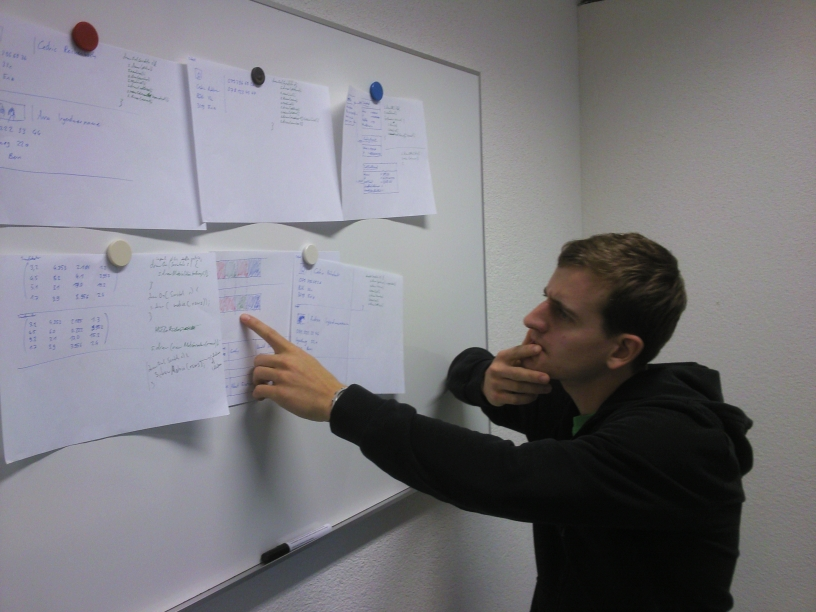
\includegraphics[width=\linewidth]{img/design-sketches_thinker.jpg}
	\caption[Confronting people with design sketches]{Programmer reacting to our sketches.}
	\figlabel{sketch-discussion}
\end{figure}

\begin{figure}[h]
	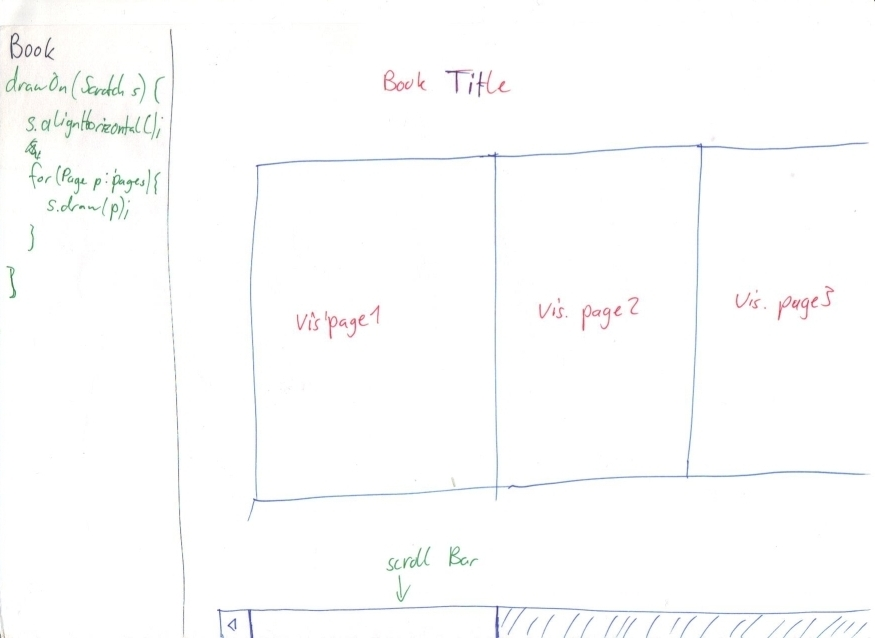
\includegraphics[width=\linewidth]{img/sketches/032.jpg}
	\caption[Bad sketch example: Horizontal and vertical alignment]{Inspired by AWT's FlowLayout, all objects are aligned horizontally.}
	\figlabel{bad-sketch_align-h-v}
\end{figure}

\begin{figure}[h]
	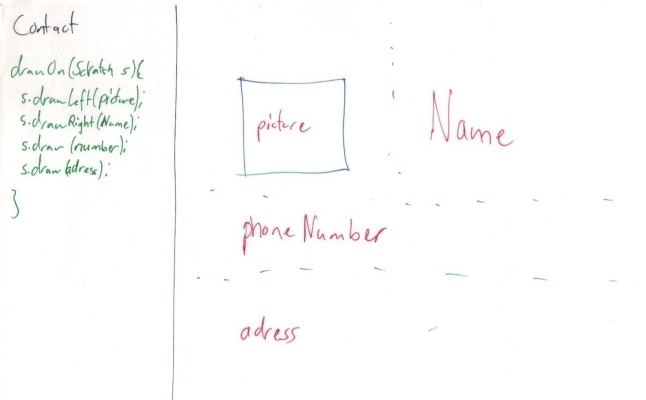
\includegraphics[width=\linewidth]{img/sketches/026.jpg}
	\caption[Bad sketch example: Left-right pattern]{A proposed canvas API that traverses the canvas from top to bottom, dividing it into virtual lines.}
	\figlabel{bad-sketch_left-right}
\end{figure}


\section{Implementation}
This section outlines the architecture and mechanisms \DD uses in order to perceive data, process them and display the results.

\subsection{Data Transport}
Since \DD is an Eclipse plugin, it's always running in a different Java VM than the project to be debugged itself.
As a consequence, object data needs to be transported after each \Doodle call.
\DD uses a third-party library\footnote{XStream, XML serializing library: \url{http://xstream.codehaus.org/}} to serialize doodled objects to XML, then transports the result as a string over a connection on localhost using SIMON\footnote{SIMON, Simple Invocation of Methods Over Network: \url{http://dev.root1.de/projects/simon}}.

\subsection{Rendering}
After a request for doodling an object has been received, \DD analyzes its type and searches for a fitting rendering in the different customization layers.
If none is available, a default rendering is used.

\subsubsection{Traversing Object Types}
Renderings are iteratively searched for all types and supertypes of an object, starting at the innermost type, defined through the object's class name.
As long as no rendering has been found, the algorithm traverses the inheritance tree in a layer-wise manner, always preferring the class type over interface types inside a layer.
In other words, this algorithm starts searching on the object's direct class and interface types, then goes on for the class' and interface's direct ancestors and repeats until a match was found or all leaves were reached.
The only type excluded from this search is the \texttt{Object} type, since it might be reached before some interface types.

\subsubsection{Output}
As output format, \DD uses HTML.
Eclipse provides the package \texttt{org.ec\-lipse.swt.brow\-ser}, which includes a web browser in the form of an Eclipse UI component.
The rendering used for this browser's content is always the one from the OS's built-in browser and cannot be changed.
As a consequence, we had to be careful when creating HTML output and always test in different browsers to prevent layout disparities on different systems.
All major changes or extensions affecting the output were tested in four Browsers with different rendering engines: Gecko (tested in Firefox), Presto (tested in Opera), Webkit (tested in Chrome) and Trident (tested in Internet Explorer).
On Windows systems, for instance, Eclipse uses the Internet Explorer rendering engine.
As a consequence, a \texttt{meta} tag needed to be set in order to suppress quirks or any other compatibility mode\footnote{MSDN documentation about legacy document modes for Internet Explorer: \url{http://msdn.microsoft.com/en-us/library/jj676915\%28v=vs.85\%29.aspx}} and make sure the newest installed rendering engine is used for best-possible support, especially for CSS3 features.


\section{Study}

\seclabel{study}
We carried out a usability study \cite{Krug00a} to validate the design of \DD.
Usability studies are qualitative rather than quantitative, offering deeper semantic insights~\cite[pp. 13--15]{Lang09b} than a quantitative study while simultaneously being easier to set up.
We posed three different problems to each test subject to be alternately solved with or without \DD, recording with screen capture videos and think aloud protocol.~\cite{Krug00a,Lang09b}
We searched for problematic situations experienced with one tool to see if they'd been solved more easily using other tools.
Seven developers solved 3 tasks each.

\subsection{Study Session Setup}
A fully functional release candidate of \DD (version 0.9.0 for Alpha and Bravo, 0.9.1 for others) was used.
It ran inside Eclipse 4.2 (Classic edition), using a ThinkPad T410 with Windows 7 (x64) and an external mouse.
The screen was captured during the whole session and one instructor sitting beside the test subject for problem explanation and protocol.
Before the actual testing, the user had 15--30 minutes to work through a tutorial and play around with \DD inside a sandbox.
At this time, the instructor was allowed to answer questions and support the subject, both on \DD and standard tools.
However, since System.out.println is a fairly basic tool, no question regarding its use came up.

For the actual session, there were 3 different small programs containing some manually inserted bug, which the subjects had to find and eliminate.
For one or two of those problems, subjects were allowed to use \DD and for the other one or two respectively, they had to fall back to classical tools (table in \ref{tool-usage-table}).
The reason for letting some subjects only use classical debugging tools was to have a reference of behavior in order to show that they are not trivial and detect what particular sub-problems they pose in detail, so we would see if \DD enables better approaches to solve them.

Subjects worked on a problem until it was completely solved, none of them needing more than 30 minutes for any particular problem.

\subsection{Subjects}
The subjects were convenience-sampled; programmers from our university and work environment were asked for participation if they had free time available. Further, they were assured of their anonymity. We informed them about the purpose of our study beforehand, and neither promised nor gave any reward for participating. The participants are enumerated in order of their participation.

\begin{tabular}{l | l | l}
Alias & Degree & Current activity \\
\hline
% Oskar Truffer
Alpha & BSc in Mathematics & Master student in CS  \\
% Remo Diethelm
Bravo & BSc in CS & Master student in CS \\
% Andrei Chis
Charlie & MSc in CS & PhD student in CS \\
% Julian Schelker
Delta & BSc in CS & Master student in CS \\
% Raffael Krebs
Echo* & MSc in CS & Industry (1 year)\\
% Roger Kohler
Foxtrot & BSc in CS & Master student in CS \\
% Ueli Scheidegger
Golf & Lic.rer.pol. in Economics & Industry (15 years)\\
\end{tabular}

*Experience with Eclipse plugin development. \\
CS: Computer Science

\subsection{Posed Problems}
In the first two tasks, the participants are given a failing unit-like test. They are informed that the test is correct, and asked to fix the bug and thus have the test pass. Subjects have access to all of the source code and are allowed to manipulate it.
While the posed problems might seem biased towards \DD, that doesn't distract from their demonstration that \DD \emph{can} vastly outperform \println. \DD, being a generalization of \println, at worst performs on par with \println.
Furthermore, not claiming that those problems are certainly best representatives of usual programming tasks, we still assume they're realistic enough to potentially occur once in a while during a programmers life.

\subsubsection{Sorting}
A couple of gray scale \texttt{Color} objects are put into a \texttt{List}
and then sorted using a custom \texttt{ColorComparator}, which should sort by brightness.
The result then is compared in a unit test to a hand-built \texttt{List} which initially has the expected order.

\paragraph{Bug and Solution}
In the comparator, completely black colors are wrongly treated as complete white.
It's an in-line case distinction that has to be adjusted.

\subsubsection{Serialization}
Phone book contacts are modeled using \texttt{Con\-tact} and \texttt{Address}  objects.
They should be serialized using a \texttt{Ser\-ializ\-ing\-Util} (simulated serialization only) and de-serialized afterwards.
In a unit test, comparison of a contact object before and after serialization fails.\\

\paragraph{Bug and Solution}
In the \texttt{SerializingUtil}, every field of type \texttt{long} is cast % NB: not "casted"
into an \texttt{integer} before serialization and back into a \texttt{long} afterwards.
This causes a field called \texttt{phoneNumber} of \texttt{Address} to be changed into a negative value.
The solution is to remove those casting operations from the code.

\subsubsection{Decimal Alignment}
In the third and last task, a class \texttt{DatabaseUtil} is given without source code, as a black box simulating access to an imaginary database by returning a two-dimensional array of \texttt{float}s when calling its only method \texttt{getData()}.
Subjects are informed that in the returned table there are duplicated tuples and have to identify them.
Finding the bug is not part of this task.

\subsection{Observed behavior}
For four study subjects, \texttt{toString()} was used as the default rendering.
Two of them, Bravo and Delta, were allowed to use \DD for solving the serialization problem and both implemented \texttt{Doodleable} with \texttt{Contact} and \texttt{Address}.
For three subjects, the ObjectDoodler (which shows all instance variables) was the standard rendering.

\begin{tabular}{l | c c c}
\label{tool-usage-table}
 & \textbf{Sorting} & \textbf{Serialization} & \textbf{Table} \\
\hline
Alpha & DD & Classic & - \\
Bravo & Classic & DD & - \\
Charlie & DD & Classic & DD \\
Delta & Classic & DD & Classic \\
Echo & DD & Classic & DD \\
Foxtrot & Classic & DD & Classic \\
Golf & DD & Classic & DD \\
\end{tabular}

\subsubsection{Observations using System.out.println}
5 out of 7 subjects (all except Delta and Echo) made use of this mechanism to visualize runtime data.
Alpha brought forward the argument of laziness to open a debugger or to stare at foreign code.
When quizzed, Alpha said they can compare things, either two different objects as posed in the sorting problem or the same object at different points in time, as in the Serialization problem.
Both are not directly possible with a classical debugger like the one built into Eclipse classic.

\paragraph{Homogenous Output}
Apart from Charlie, none of the subjects spent time customizing their ad-hoc textual prints by overriding \texttt{toString} on objects to be visualized.
If any, they utilized in-line string concatenation for formatting purposes, like inserting delimiters between different objects.
Beta printed each element of the wrongly sorted color list and then stared at the (unaligned) numerical values of red, green and blue color components.
Once he found out that a black element was at the end instead of the beginning, he went on to investigate the cause, leading to the problem.

In contrast, subjects using \DD already had built-in renderings for \texttt{Collection}  and \texttt{Color}, making the problem immediately obvious.

\paragraph{Uninspectable and Useless Output}
The standard implementation of \println prints only the class name and object hash, for example:
\begin{lstlisting}
ch.unibe.scg.spacepirates.Player@ece88d2
\end{lstlisting}
Bravo and Golf resorted to a compile-run cycle, where they would explore the object graph by re-running the program, adapting the print statement to explore the parts of the object graph they were interested in.

Charlie was the only subject to override \texttt{toString} methods, after being dissatisfied with the standard printout of class name plus hash. He implemented \texttt{toString}  to print out all fields of an object, as seen in \Figref{charlie-toString}.
He argued that the difference between two states of an object should be visible when seeing all its field, recursively including fields of referenced objects.

\begin{figure}[h]
\begin{lstlisting}
public class Contact { ...
  public String toString() {
	return "name: " + name
		+ ", address: " + address;
  }
}
public class Address { ...
  public String toString() {
	return "street: " + street
	  + ", phoneNumber: " + phoneNumber
	  + ", city: " + city;
  }
}
\end{lstlisting}
  \caption{Charlie overwrote \texttt{toString()} to aid debugging.}
  \figlabel{charlie-toString}
\end{figure}

Alpha produced a very similar output, but instead of overriding \texttt{toString()}, he extracted all fields from outside using getter methods directly inside the \println method (\figref{alpha-println}).

\begin{figure}[h]
\begin{lstlisting}
System.out.println("name: " + contact.getName()
		+ ", street: "
		+ contact.getAddress().getStreet()
		+ ", phoneNumber: "
		+ contact.getAddress().getPhoneNumber()
		+ ", city: "
		+ contact.getAddress().getCity();
\end{lstlisting}
  \caption{Alpha used \texttt{\println} to aid debugging.}
  \figlabel{alpha-println}
\end{figure}

Another approach to solve insufficient output was to switch from \println to the debugger, observed with Bravo and Foxtrot.

\subsubsection{Observations using a Debugger}
Four subjects (Bravo, Delta, Echo and Foxtrot) used the Eclipse debugger to inspect objects, only Delta and Echo using it exclusively.
Echo's argumentation for this usage was that debuggers are more powerful in comparison to \println, because they allow one to inspect objects dynamically and additionally provide simple improvements of standard textual representations (\eg arrays are represented in the form of \texttt{[objectA, objectB, ...]}instead of \texttt{[Ljava.lang.Object;@4cb162d5}.
Echo mentioned that they missed the feature to compare two objects from different points in time.

\paragraph{Comparison Between Objects}
The built-in Eclipse debugger only allows you to inspect one object at one point in time.
As the serialization problem consists of two objects unexpectedly  being unequal, part of the debugging process was somehow comparing them in order to find their difference.
Every subject except Golf did this --- Golf only tried to understand the serialization and de-serialization process to find out where the implementation has mistakes.
Echo never used \println, but attempted to compare objects before and after serialization using the debugger.
Even though the debugger supported simple and fast inspection to any point inside the object, Echo explicitly pointed out that he missed the feature to inspect two objects simultaneously.

\paragraph{Non-Selective Output}
Eclipse's Java debugger simply lists all contents of an object, since there is no information about relevance of its respective parts.
The debugger is working at runtime and therefore only knows the instantiated type of an object, so it will visualize all properties and contents of this, potentially resulting in a overly verbose output.
In particular, programmers only interacting with an object over some super type may have a much simpler mental model of what it is than represented in the debugger on the basis of its runtime type.
We observed this in the color list problem, where \texttt{ArrayList}
was used as implementation for the interface \texttt{List}.
Subject Bravo initially tried to perceive the structure of a list right after sorting by pausing the program  using the debugger and inspecting the mentioned list (\Figref{debugger_color-list}), but instantly gave up and switched to writing a \texttt{for} loop which sequentially prints out all elements using \println.

\begin{figure}[h]
	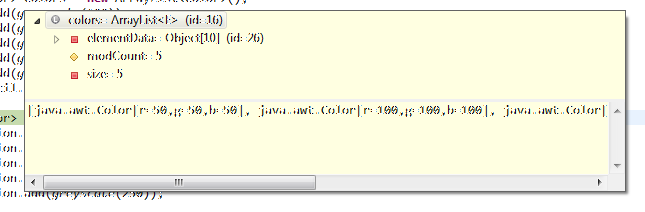
\includegraphics[width=\linewidth]{img/debugger_color-list_remo.png}
	\caption[Bravo using the debugger for a color list]{Eclipse's debugger visualizes all fields of an object's runtime type (ArrayList)}
	\figlabel{debugger_color-list}
\end{figure}

\subsubsection{Observations using \DD}
When allowed (but not forced) to use \DD, every subject solved the problem without making use of any other tool.
Only two subjects ever implemented the \texttt{Doodleable} interface for solving a problem.
Based on their implementation and \texttt{toString} implementations of other subjects, we changed the default object rendering from using \texttt{toString} to listing all instance variables.
As a consequence, subjects found relevant information directly after doodling an object, making any customization unnecessary.

\paragraph{Two methods in \texttt{Doodleable} interface}
Echo was confused about the difference between the two methods in the \texttt{Doodleable} interface. After going back to the documentation of the interface, he understood.
Alpha did not show any reaction when implementing the \texttt{Doodleable} interface, but misunderstood the meaning of its two methods: Instead of reducing the number of objects on the canvas, he simply delegated the zoom mechanism to each one by using the \texttt{Canvas.drawSmall} method (\figref{wrong-doodleable-usage}).

Since none of the other subjects ever made used of \texttt{Canvas.drawSmall} and Alpha misunderstood its purpose, we removed this method from the API.

\begin{figure}[h]
\begin{lstlisting}
public void doodleOn(Canvas c) {
	c.draw(name);
	c.newLine();
	c.draw(phoneNumber);
	c.newColumn();
	c.draw(address);
}
public void summarizeOn(Canvas c) {
	c.drawSmall(name);
	c.newLine();
	c.drawSmall(phoneNumber);
	c.newColumn();
	c.drawSmall(address);
}
\end{lstlisting}
  \caption{Alpha mistakenly delegated the zooming mechanism to each printed object.}
  \figlabel{wrong-doodleable-usage}
\end{figure}

\paragraph{Console Keeps Stealing Focus}
\seclabel{console-focus-problem}
When certain output is printed onto the Eclipse console, it gains the UI's focus by default.
Due to the problem setup, every program initially threw an exception at the end of its execution, signaling the problem had not been solved yet.
Every user experienced the following problem at least once: They were using \DD and therefore had this view tab opened when the exception was thrown and Eclipse switched to the console.
Only Echo managed to disable its focus-on-change setting, while the other subjects just switched back to the \DD view tab after a few seconds.

\paragraph{Problem immediately obvious}
Charlie doodled both the wrongly sorted color list and the correctly sorted one. Since they were both on-screen immediately, he instantly noticed both their similarity and the difference, which was that the black color was on the wrong side of one list.

On the serialization problem, all three subjects (Bravo, Delta, Foxtrot) using \DD managed to find the changed field instantly after calling \texttt{Doo.dle()} once before and once after the de-/serialization step. That's because \DD's \texttt{ObjectPlugin} shows all instance variables, which was enough to immediately see the problem.

\paragraph{Default doodles were useless}
When Alpha used the default visualization without implementing the \texttt{Doodleable} interface, \DD simply defaulted to printing
the output of the \texttt{toString()} method. This was entirely useless, as it only printed the name of class plus an object hash.
Thus, Alpha implemented the \texttt{Doodleable} interface, and included all instance variables of the questioned object for its representation.

On sessions without \DD, Golf iteratively re-ran the program, each time printing another field of the same object and Bravo wrote a custom textual representation, printing all fields labelled with their names.

Based on these findings, we modified \DD's standard rendering: Instead of falling back to the object's \texttt{toString()} method, the new default rendering prints all fields, including field name, as seen in \Figref{fielddoodler-player}.

\subsubsection{Observations Without Any Debugging Tool}
Subject Golf was the only one to solve a problem without using any debugging tool.
On the serialization problem, he tried to comprehend the logic of the problem's \texttt{SerializingUtil}.
Unlike others, he found the problem source at the same time as the nature of the problem itself.
He fixed the bug and verified the result using \println.


\section{Future Work}

\paragraph{Highlighting Object Diffs}
When tracking an object over time, the most important information is located where properties of an object have changed.
Therefore, a mechanism comparing objects when they are doodled multiple times could be a powerful feature.

\paragraph{Clickable Doodles}
One problem of using \println over a long period of time is that it's indeed clear which object is printed, but not where the \println call has been made.
To find it, some tedious text search over the whole project is needed in the worst case.
As a solution in \DD, doodles could include a link pointing to the line in source code where the \Doodle call was triggered, similar to the way Throwables are tracked.

\paragraph{Debugger Integration}
Since the eclipse debugger only uses textual representations and doesn't allow any customization, a way to enhance it could be to include doodles.
A user would be allowed to switch from the standard textual mode to \DD mode, where an object would be inspected using \DD's rendering.
Or a button beside the textual representation would create a popup with the doodled version of it.

\section{Related Work}
\subsection{Existing Debugging Tools}
In the world of programming languages, there are two classes of widely used debugging tools:
Textual output like Java's \println and Debuggers.

\subsubsection{Textual Output}
Java's \println provides a default textual representation for any object.
Primitives and Strings are rendered in a trivial way; all other objects, including arrays, are represented with their class name and object hash.
Any object's representation can be changed by overriding its \texttt{toString} method.

Debugging by directly writing into source code may be easier and quicker than having to equip other debugging tools for a session\cite[p. 119]{Kern99a}.
Also, objects can be tracked over time by printing them at different points of execution and comparing the resulting outputs.

\paragraph{Best Practice For Textual Output}
To understand in detail how programmers use textual output for debugging, we wrote a script that searches for such methods in open source projects.
It analyzed SqueakSource, a hosting service for Smalltalk projects, searching for \texttt{printOn} methods, Smalltalk's equivalent to Java's \println.
Achieved results\cite{Schw11b} gave us hints on how to design default renderings on the one hand and showed shortcomings of text-only output.

\paragraph{Missing Features On Textual Output}
To achieve two-dimensional renderings in text, the developer only has the newline character as an option.
Since a line can have only one new-line character, putting two 2-dimensional structures next to each other requires coordination. In practice, developers instead refrain from printing 2-dimensional structures next to each other~\cite{Schw11b}, and instead print them below each other, as illustrated in \Figref{nested-matrix-problem}.
Furthermore, the resulting output is purely static, and offers no possibility to navigate to related objects or back to the source code.

\begin{figure}[h]
	\begin{lstlisting}
	an Array(
	MatrixTransform2x3(
		2.0 0.0 0.0
		0.0 2.0 0.0
	) MatrixTransform2x3(
		1 -0.707107 0.0
		0.707107 0.707107 0.0
	))
	\end{lstlisting}
	\caption{Textual visualization of an array of 2D-matrices, without DoodleDebug.}
	\figlabel{nested-matrix-problem}
\end{figure}

\subsubsection{Debuggers}
Debuggers allow users to stop a program's execution at any line of source code.
When stopped, any detail of the current state is inspectable.
Unlike \println, debuggers allow their users to put additional or remove existing break points at runtime, which makes changing the target piece of code to debug quicker, especially because the current program state doesn't need to be re-created like on a new run.

\paragraph{Drawbacks Of Using A Debugger}
Since a debugger only shows the program's state at one point in time, comparison of two time slices is hardly possible.
Important details may only be memorized and mentally compared to the ones at a later point in time.

Eclipse's built-in Java debugger brings no options to customize its output.
When inspecting an object, all its fields are listed by name, together with a textual representation.
An object containing many fields may be costly to inspect if only few of them are relevant to the current user.


\section{Conclusion}
\DD is a valuable drop-in replacement for Java's \println.
It introduces techniques to enhance debugging output by adopting well-proven mechanisms from debuggers and console printing on the one hand and introducing simple new ones on the other hand.
Getting started is rather easy since one single API method already enables the core features of \DD.
Previous \println statements can be directly replaced by \Doodle calls without losing any ground.

Since the output is held in HTML and \DD is bound to be an Eclipse plugin, the possibilities for additional features are infinite.
The output view with JavaScript running in it is Turing-complete and supports any graphical output a monitor can display.
Any IDE-related actions can be implemented because a stable communication between output and plugin code is already running.

The DoodleDebug Eclipse plugin, all source code and a demo video are available at \url{http://scg.unibe.ch/wiki/projects/DoodleDebug}.

\section{Acknowledgements}
I'm not good with speeches.
But I can truly say that the following people didn't fear to face any possible effort while accompanying me on this journey, thank you:
Niko Schwarz, Oscar Nierstrasz, Mirca Lungu, Andrei Chief, the SCG, and all study participants.


\bibliographystyle{plain}
\bibliography{bib/scg}{}

\end{document}